\chapter{Evolution and Uses of Code Generation in C\#}

This thesis aims to enhance the runtime performance of ASP.NET Core applications by developing a new action discovery using C\# source generators. This approach, which involves generating static code, potentially leads to more efficient and scalable web applications.

This chapter provides a comprehensive look at the evolution and use of code generation techniques in C\#. We start with exploring the difference between runtime and static code generation before diving into the more modern tools such as the Roslyn API and source generators. We then look at how source generators are used in everyday development tasks, including serialization, logging, dependency injection, and ASP.NET Core routing, highlighting their role in improving code performance and maintainability. The chapter also discusses the limitations and challenges of source generators, offering a balanced perspective on this innovative technology in the .NET ecosystem.

\section{Overview of Code Generation Techniques}

Code generation techniques encompass a range of strategies for creating code automatically or semi-automatically. These techniques can improve the development process by automating repetitive tasks, enhancing code quality, and optimizing performance. This section will explore different techniques, including runtime code generation, static code generation, and reflection. The benefits and drawbacks of each will be discussed, providing a comprehensive understanding of their applicability in different scenarios.

\subsection{Runtime Code Generation}

Runtime code generation, also known as dynamic code generation, is a technique where code is generated and executed during the runtime of a program. This approach enables developers to create code that adapts to the current execution context, allowing for more flexibility and customization. Runtime code generation can be employed in various scenarios, such as creating specialized implementations of algorithms or generating code based on user input or configuration data\cite{Chiba1995, Aycock2003}.

One standard method for achieving runtime code generation is Just-In-Time (JIT) compilation. JIT compilers translate portions of code, typically bytecode or intermediate language (IL) code, into machine code during the execution of a program\cite{Aycock2003}. This technique allows for optimizations based on the specific runtime environment, such as hardware characteristics or runtime data\cite{Gal2006}. The .NET runtime, for instance, employs a JIT compiler to compile the Common Intermediate Language (CIL) code into native code during the execution of a .NET application\cite{Esposito2014}.

\subsection{Reflection in Runtime Behavior Customization}

Reflection is a mechanism that allows a program to analyze and manipulate its structure and behavior during execution \cite{Maes1987}. In C\#, reflection can inspect the metadata of types and members, create instances of types, invoke methods, and access fields and properties dynamically \cite{Albahari2019}. This enables developers to write code that can adapt its behavior based on this metadata information at runtime. While reflection provides a powerful and flexible means of customizing program behavior during runtime, it can introduce performance overhead due to the need to analyze and manipulate the metadata of the executing assembly \cite{Skeet2019, Tudose2013}.

Using runtime behavior customization techniques such as reflection can offer several advantages, such as increased flexibility, adaptability, and the ability to perform optimizations based on runtime information\cite{Chiba1995, Aycock2003}. However, there are also potential drawbacks, including increased complexity, potential security risks, and performance overhead\cite{Aycock2003, Pobar2005, Tudose2013}. In particular, the performance impact of runtime code generation is a significant concern when discovering the actions in an ASP.NET Core application.

\subsection{Static Code Generation}

Static code generation refers to generating code at compile time before the application is executed. This approach is in contrast to runtime code generation, which occurs during the execution of an application. With static code generation, the generated code is combined with the source code during compilation, resulting in a single executable binary. This technique offers several advantages, including better performance, improved type safety, and easier debugging in some scenarios \cite{Chiba2000}.

Static code generation has improved software performance and maintainability in various contexts. For instance, in web development, static site generators like Jekyll and Hugo produce HTML, CSS, and JavaScript files at build time rather than generating them on-the-fly for each request \cite{Biilmann2015}. This approach can improve performance and security, as a simple web server can serve the generated content without needing server-side processing.

One of the most common approaches to static code generation is metaprogramming, where code is generated or transformed by other code \cite{Cordy1992}. Various programming languages, including Lisp, Haskell, and C++, provide mechanisms for metaprogramming, such as macros, templates, or code generation tools \cite{Cordy1992}. In the context of C\#, source generators are a relatively recent addition to the language that enables static code generation by analyzing the existing code and generating new source code during the compilation process \cite{Microsoft2022SourceGenerators}.

Static code generation can also be achieved using code generation tools and libraries. For example, tools like the Java Architecture for XML Binding (JAXB) and the .NET Framework's Windows Communication Foundation (WCF) generate code from XML schemas or interface definitions, respectively \cite{Vogel2023, Microsoft2021WhatLearn}. These tools help reduce the manual code developers must write and maintain, making keeping the codebase consistent with the underlying data structures or interfaces easier.

While static code generation offers numerous benefits, it also has some drawbacks. One of the main challenges is the increased complexity of the build process, as the code generation tools and libraries need to be integrated into the build pipeline. Additionally, the generated code may be less readable or harder to debug, as it may not directly correspond to the source code or follow established coding conventions \cite{Chiba2000}.


\section{Evolution of C\# and Code Generation}

As C\# and the .NET ecosystem have evolved, various code-generation techniques have been developed and integrated into the platform. This section will discuss three significant milestones in the evolution of C\# code generation: T4 templates, the Roslyn API, and the introduction of source generators. Each milestone represents a step forward in how developers can generate and manipulate code in C\# applications, providing more efficient and sophisticated methods for managing complex projects. Understanding the context and limitations of each technique is essential for appreciating the current state of code generation in C\# and the role of source generators in addressing the challenges of previous approaches.

\subsection{T4 Templates and their Limitations}

Text Template Transformation Toolkit (T4) is a code generation technology that has been a part of the .NET ecosystem since the release of Visual Studio 2005\cite{Klein2010}. T4 templates are text-based templates that allow developers to generate code using a mixture of static text, control logic, and data from external sources \cite{Klein2010}. T4 has been widely used in various scenarios, including generating code for data access layers, model-driven development, and code scaffolding \cite{Vogel2010}.

However, T4 templates have limitations that make them less suitable for specific code-generation tasks. One of the primary drawbacks of T4 templates is that they lack real-time execution \cite{Klein2010}. This means that the T4 templates only transform when you save the template file or when one manually initiates the transformation. They do not automatically update when the data they depend on changes, which can lead to outdated output \cite{Klein2010}. Furthermore, T4 templates do not provide any means to validate the generated code during the generation process, which can lead to syntax errors or other issues in the generated code that may not be detected until the code is compiled \cite{Vogel2010}.

Another limitation of T4 templates is that they do not support direct unit testing \cite{Klein2010}. Since the templates are not C\# Code, they can not be tested with the same unit testing framework as the rest of the project. Instead, one would have to transform the templates and test the outcome. Additionally, one of the most significant drawbacks of T4 templates is the lack of a robust mechanism for integrating with the C\# language features and the compiler, which can make it challenging to achieve advanced code generation scenarios or leverage the full power of the C\# language in generated code \cite{Esposito2014}.

These limitations have led to exploring alternative code generation techniques within the C\# and .NET communities, with the Roslyn API and source generators emerging as more advanced and flexible solutions for code generation tasks.

\subsection{Roslyn API}

The Roslyn API, introduced by Microsoft in 2011, is a set of open-source compilers and code analysis APIs for C\# and Visual Basic .NET (VB.NET) languages \cite{CSharpRoslyn}. Roslyn's primary goal is to enable developers to write custom tools and analyzers, providing a deep understanding of the source code by exposing its syntax trees, symbols, and semantic information \cite{Vermeir2022}. The API is designed to be language- and platform-agnostic, which makes it suitable for various use cases, such as code analysis, refactoring, and code generation \cite{Vermeir2022}.

One of Roslyn's significant advantages is its ability to perform real-time code analysis. This feature allows developers to identify potential issues and opportunities for refactoring as they write code, significantly reducing the time spent on manual code reviews \cite{Vermeir2022}. Furthermore, Roslyn provides a platform for developers to create custom diagnostics and refactorings, which can be easily integrated into IDEs like Visual Studio, enabling a more streamlined development process \cite{CSharpRoslyn}.

Although Roslyn offers many benefits over T4 templates, it has limitations. While Roslyn is excellent for code analysis and refactoring, it is not designed explicitly for code generation like T4 templates \cite{Vermeir2022}. However, with the introduction of source generators in C\# 9, this gap has been addressed, allowing developers to leverage the power of Roslyn for code generation tasks as well \cite{Carter2020}.

\subsection{Introudction of Source Generators}

The introduction of source generators in C\# 9 offers developers a novel method for executing compile-time code generation in .NET applications, thus overcoming the limitations associated with runtime code generation and T4 templates \cite{Torgersen2020}. As shown in Figure \ref{fig:source_generators_workflow}, source generators are part of the normal compilation process.

\begin{figure}[H]
\centering
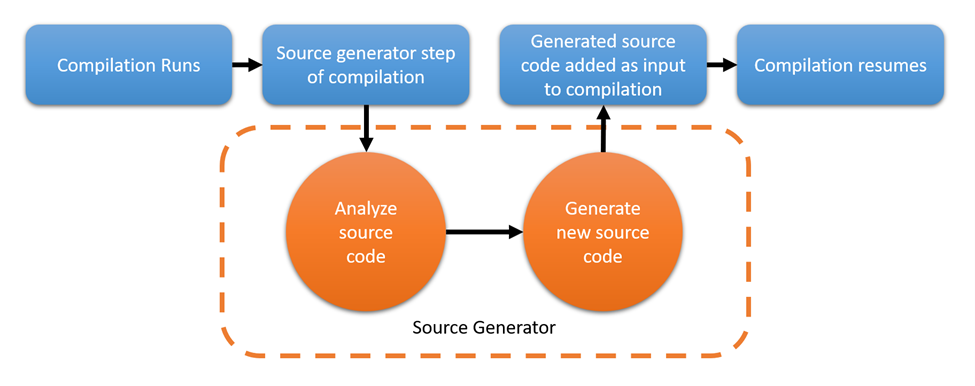
\includegraphics[width=0.8\textwidth]{graphics/source-generator-visualization.png}
\caption{Source Generators Overview}
\label{fig:source_generators_workflow}
\end{figure}

The figure above illustrates the integration of source generators in the C\# compilation process. It commences with the running of the compilation, which then transitions to the source generator step. This segment involves two fundamental operations: "Analyze source code" and "Generate new source code." The analyzed code provides information that the source generators use to produce new source code. Once the source generator completes these tasks, the generated source code is added back as input to the compilation process. Following this addition, the compilation process resumes, thus concluding the sequence \cite{CSharpRoslyn}.

The Roslyn API provides source generators with access to both the abstract syntax tree (AST) and the semantic model of the code under compilation \cite{CSharpRoslyn}. The AST represents the syntactic structure of the source code, breaking it down into a tree-like form that encapsulates the source code's grammatical structure \cite{CSharpRoslyn}. The semantic model, on the other hand, captures the meaning of the code, encapsulating information about variables, types, scope, and more \cite{CSharpRoslyn}.

This access to syntax and semantics empowers source generators to create code that naturally integrates with the original source \cite{CSharpRoslyn}. The generated code can interact seamlessly with the handwritten code, all while upholding type safety and other compile-time checks \cite{Carter2020}. This unique combination of integration and safety significantly improves the code generation process within the .NET ecosystem.

Source generators also pioneer new prospects for code optimization and performance improvements. By generating code during compile-time, source generators can reduce the need for resource-demanding runtime operations, thus providing a more performance-efficient alternative for code generation tasks \cite{CSharpRoslyn}.

The emergence of source generators has stimulated innovation and encouraged the development of new tools and libraries in the .NET ecosystem. Developers' growing adoption of source generators is leading to the creation of an increasing number of libraries and tools that facilitate and simplify the code generation process. This flourishing ecosystem underscores the utility of source generators in contemporary .NET development, granting developers a potent, performant, and user-friendly mechanism for generating code at compile-time.

\section{Use Cases and Applications of Source Generators}

Source generators, a recent addition to the C\# language and .NET platform, are potential game changers for application performance, maintainability, and robustness. This section briefly reviews four primary use cases: serialization, logging, dependency injection, and ASP.NET Core routing, highlighting how source generators can overcome the limitations of the current implementations.

\subsection{Serialization}

Serialization involves converting an object's state into a format suitable for storage or transmission and is a routine procedure in C\# and the .NET ecosystem \cite{Fowler2002}. Traditional .NET serialization libraries often rely on runtime reflection, which can lead to performance overheads \cite{NewtonsoftJsonPerformance, Tudose2013}. Source generators provide a resolution by enabling serialization code generation at compile-time, thus eliminating the need for runtime reflection and improving performance \cite{CSharpRoslyn}. Libraries like System.Text.Json have already adopted source generators to optimize serialization performance in .NET \cite{SystemTextJson, SystemTextJsonSourceGen}.

\subsection{Logging}

Logging, a fundamental aspect of software development, enables developers to observe and analyze their applications' behavior. While numerous logging libraries are available for .NET, such as log4net, NLog, and Serilog, each comes with unique features and performance considerations. Formatting, filtering, and writing log entries to various output destinations can introduce a noticeable overhead during runtime, potentially slowing down the application \cite{Serilog, Fowler2002}.

Source generators present a new perspective on improving the efficiency of logging. By generating code at compile-time, source generators can replace costly runtime operations, such as string interpolation and method calls, enhancing application performance. They can tailor the generated code to specific logging scenarios, reducing the runtime overhead associated with logging \cite{Carter2020, Fowler2002}.

Moreover, source generators allow for static code analysis during compilation, which can identify potential issues with the logging code—like incorrect log levels or formatting—early on. By providing feedback in the form of compiler warnings or errors, source generators can contribute to more accurate and reliable logging practices \cite{Torgersen2020}.

Another advantage of using source generators in logging is simplifying configuration and setup for logging libraries. They can analyze the application code and configuration and generate tailored logging implementations specific to the application's requirements. This eliminates the need for manual configuration or complex initialization code, leading to a cleaner, more maintainable code and a streamlined development experience \cite{CSharpRoslyn}.

\subsection{Dependency Injection}

Dependency Injection (DI) is a widely-used design pattern that promotes loosely-coupled and modular software design by injecting dependencies into an object instead of having the object create them directly \cite{Martin2003}. In the .NET ecosystem, the built-in DI container and various third-party libraries, such as Autofac and Ninject, allow the use of dependency injection \cite{DIContainers}. However, dependency resolution at runtime can introduce overhead, as the DI container needs to manage and resolve dependencies, potentially affecting application performance \cite{Blumhardt2010}.

Source generators offer an opportunity to optimize the DI process by generating code for dependency resolution at compile-time \cite{CSharpRoslyn}. By analyzing the application's codebase and identifying the required dependencies, source generators can create tailored code to resolve and manage dependencies, eliminating the runtime overhead associated with dependency resolution \cite{Carter2020}. The generated code can also benefit from advanced compiler optimizations, further enhancing the performance of the DI process \cite{Torgersen2020}.

Additionally, source generators can help enforce best practices in DI configuration by analyzing the code and providing compile-time feedback on potential issues, such as missing or incorrect registrations \cite{CSharpRoslyn}. This can lead to more robust and maintainable applications by ensuring that dependency injection is correctly configured and implemented.

\subsection{ASP.NET Core Routing}

ASP.NET Core Routing, an essential component of the ASP.NET Core framework, ensures the correct mapping of incoming requests to their appropriate action methods in controllers \cite{Microsoft2023RoutingCore}. At the heart of this routing process is the action discovery, an approach that leverages runtime reflection to examine the structure of controllers, identify their methods, and access associated metadata such as route attributes \cite{Microsoft2023RoutingCore}. Despite its flexibility, this dynamic approach introduces performance overhead due to the computational expense of runtime reflection \cite{Microsoft2023RoutingCore}.

The introduction of source generators in C\# 9.0 offers a compelling approach to simplify the action discovery process. Generating static code during compilation eliminates the need for runtime reflection, making the process more efficient during the application startup phase \cite{CSharpRoslyn}. The source generators would have to examine the application's codebase, extract necessary routing information from controllers and their action methods, and generate code that summarises the extracted information \cite{Carter2020}. As a result, there is a potential for significant performance improvements, especially in applications with a large number of controllers.

Source generators also have the potential to improve the development process by providing early insights into potential issues with action discovery. For instance, if a method lacks the necessary attributes to be recognized as an action, a compile-time alert can be triggered, assisting developers in identifying and addressing such issues before deployment. This not only aids in enhancing the robustness of the web applications but also contributes to streamlining the development workflow, thereby improving overall productivity.

\section{Limitations and Challenges of Source Generators}

While introducing source generators in C\# 9 has brought about significant advancements in code generation, it is crucial to recognize that they also come with limitations.

Firstly, source generators do not modify existing code; they only add new code to the compilation. This means that developers cannot use source generators to automatically refactor or change the behavior of existing code \cite{CSharpRoslyn}. While this restriction is intended to prevent unexpected side effects and maintain the integrity of the source code, it can limit the scope of applications for source generators \cite{Carter2020}.

Secondly, source generators are executed during the compilation process; hence, their runtime is included in the overall compile time of the application \cite{CSharpRoslyn}. As a result, poorly optimized source generators can significantly increase compile times, affecting the developer experience, particularly in large codebases \cite{Carter2020}.

Furthermore, source generators work on a syntax tree representation of the code, meaning they cannot access the results of previous compiler phases, such as constant folding or definite assignment analysis \cite{Torgersen2020}. This can make specific code generation tasks more complex or even impossible in some cases \cite{CSharpRoslyn}.

Lastly, while source generators have the potential to significantly improve the performance of applications by moving computation from runtime to compile-time, they also require developers to think in a new paradigm. This could potentially increase the complexity of the code and require a learning curve for developers new to the concept of metaprogramming \cite{CSharpRoslyn}.